\documentclass[12pt]{article}
\usepackage[margin=1in]{geometry}
\usepackage{amsmath, amssymb, bm}
\usepackage{fancyhdr}
\usepackage{enumitem}
\usepackage{graphicx}
\usepackage{float}

% --- Header / Footer Setup ---
\pagestyle{fancy}
\fancyhf{}
\lhead{Tyler Jones}
\chead{ME 563: HW 1}
\rhead{University of Wisconsin--Madison}
\cfoot{\thepage}

% --- Custom Commands ---
\newcommand{\pd}[2]{\frac{\partial #1}{\partial #2}}

\begin{document}

\section*{Problem 1}
\textbf{Consider a pump designed for incompressible liquids. The pump is characterized by impeller diameter $d$ and spins at constant angular velocity $\Omega$. Liquid of density $\rho$ enters the pump at pressure $P_1$ and discharges at pressure $P_2$. Neglecting viscosity, perform a dimensional analysis relating the nondimensional pressure rise across the pump to the other variables, plot the given data in nondimensional form, and comment on whether the analysis identified the correct nondimensional relationship.}

\begin{figure}[H]
    \centering
    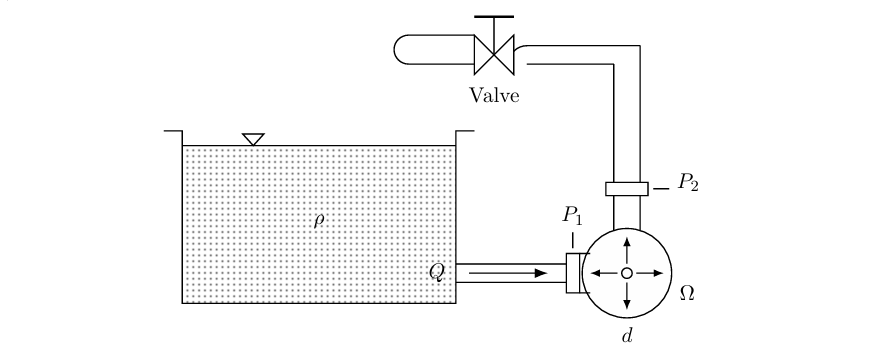
\includegraphics[width=0.7\textwidth]{../figures/me563_hw1_p1.png}
    \label{fig:pump_schematic}
\end{figure}

\subsection*{Part (a)}
\textbf{Perform dimensional analysis to determine the nondimensional relation between nondimensional pressure rise across the pump and the other variables.}

Let $\Delta P = P_2 - P_1$ denote the pressure rise across the pump. Neglecting viscosity, we assume
\begin{equation*}
    \Delta P = f(\rho, Q, \Omega, d)
\end{equation*}
The fundamental dimensions of the variables are:
\begin{itemize}[noitemsep]
    \item $[\Delta P] = M L^{-1} T^{-2}$
    \item $[\rho] = M L^{-3}$
    \item $[Q] = L^3 T^{-1}$
    \item $[\Omega] = T^{-1}$
    \item $[d] = L$
\end{itemize}

With $N = 5$ variables and 3 fundamental dimensions ($M, L, T$), the dimensional matrix has rank $R = 3$, giving $N - R = 2$ dimensionless groups. Choosing $\rho, \Omega, d$ as repeating variables:

For $\Pi_1$, containing $\Delta P$:
\begin{align*}
    \Pi_1 &= \Delta P\, \rho^a \Omega^b d^c \\
    M^0 L^0 T^0 &= (M L^{-1} T^{-2})(M L^{-3})^a (T^{-1})^b (L)^c
\end{align*}
Matching exponents:
\begin{align*}
    M:&\ 1 + a = 0 \implies a = -1 \\
    L:&\ -1 - 3a + c = 0 \implies c = -2 \\
    T:&\ -2 - b = 0 \implies b = -2
\end{align*}
\begin{equation}
    \Pi_1 = \Delta P\, \rho^{-1} \Omega^{-2} d^{-2} = \frac{\Delta P}{\rho \Omega^2 d^2}
\end{equation}

For $\Pi_2$, containing $Q$:
\begin{align*}
    M:&\ a = 0 \\
    L:&\ 3 - 3a + c = 0 \implies c = -3 \\
    T:&\ -1 - b = 0 \implies b = -1
\end{align*}
\begin{equation}
    \Pi_2 = Q\, \Omega^{-1} d^{-3} = \frac{Q}{\Omega d^3}
\end{equation}

By the Buckingham Pi theorem, $\Pi_1 = f(\Pi_2)$:
\begin{equation}
    \frac{\Delta P}{\rho \Omega^2 d^2} = f\left(\frac{Q}{\Omega d^3}\right)
\end{equation}
Defining the pump head as $H \equiv \Delta P / (\rho g)$, this becomes
\begin{equation}
    \frac{gH}{\Omega^2 d^2} = f\left(\frac{Q}{\Omega d^3}\right)
\end{equation}
i.e. the head coefficient $\psi = gH/(\Omega^2 d^2)$ is a function of the flow coefficient $\phi = Q/(\Omega d^3)$.

\subsection*{Part (b)}
\textbf{Plot the data in the table in non-dimensional form using the non-dimensional variables determined in part (a).}

The flow rate and head data at each of the three pump speeds (1000, 1475, and 1990 rpm) were converted to SI units (gpm $\to$ m$^3$/s, ft $\to$ m, rpm $\to$ rad/s) and combined with $g = 9.81 \text{ m/s}^2$ to compute $\phi = Q/(\Omega d^3)$ and $\psi = gH/(\Omega^2 d^2)$ for every data point. The impeller diameter $d$ is not given in the problem; since the same physical pump ($d = \text{const}$) is used at all three speeds, an arbitrary but consistent value of $d$ only rescales both axes uniformly and does not affect whether the three speed curves collapse onto a single curve, so $d = 1$ was used as a placeholder. The resulting nondimensional performance curves are shown in Figure~\ref{fig:pump_nondim}.

\begin{figure}[H]
    \centering
    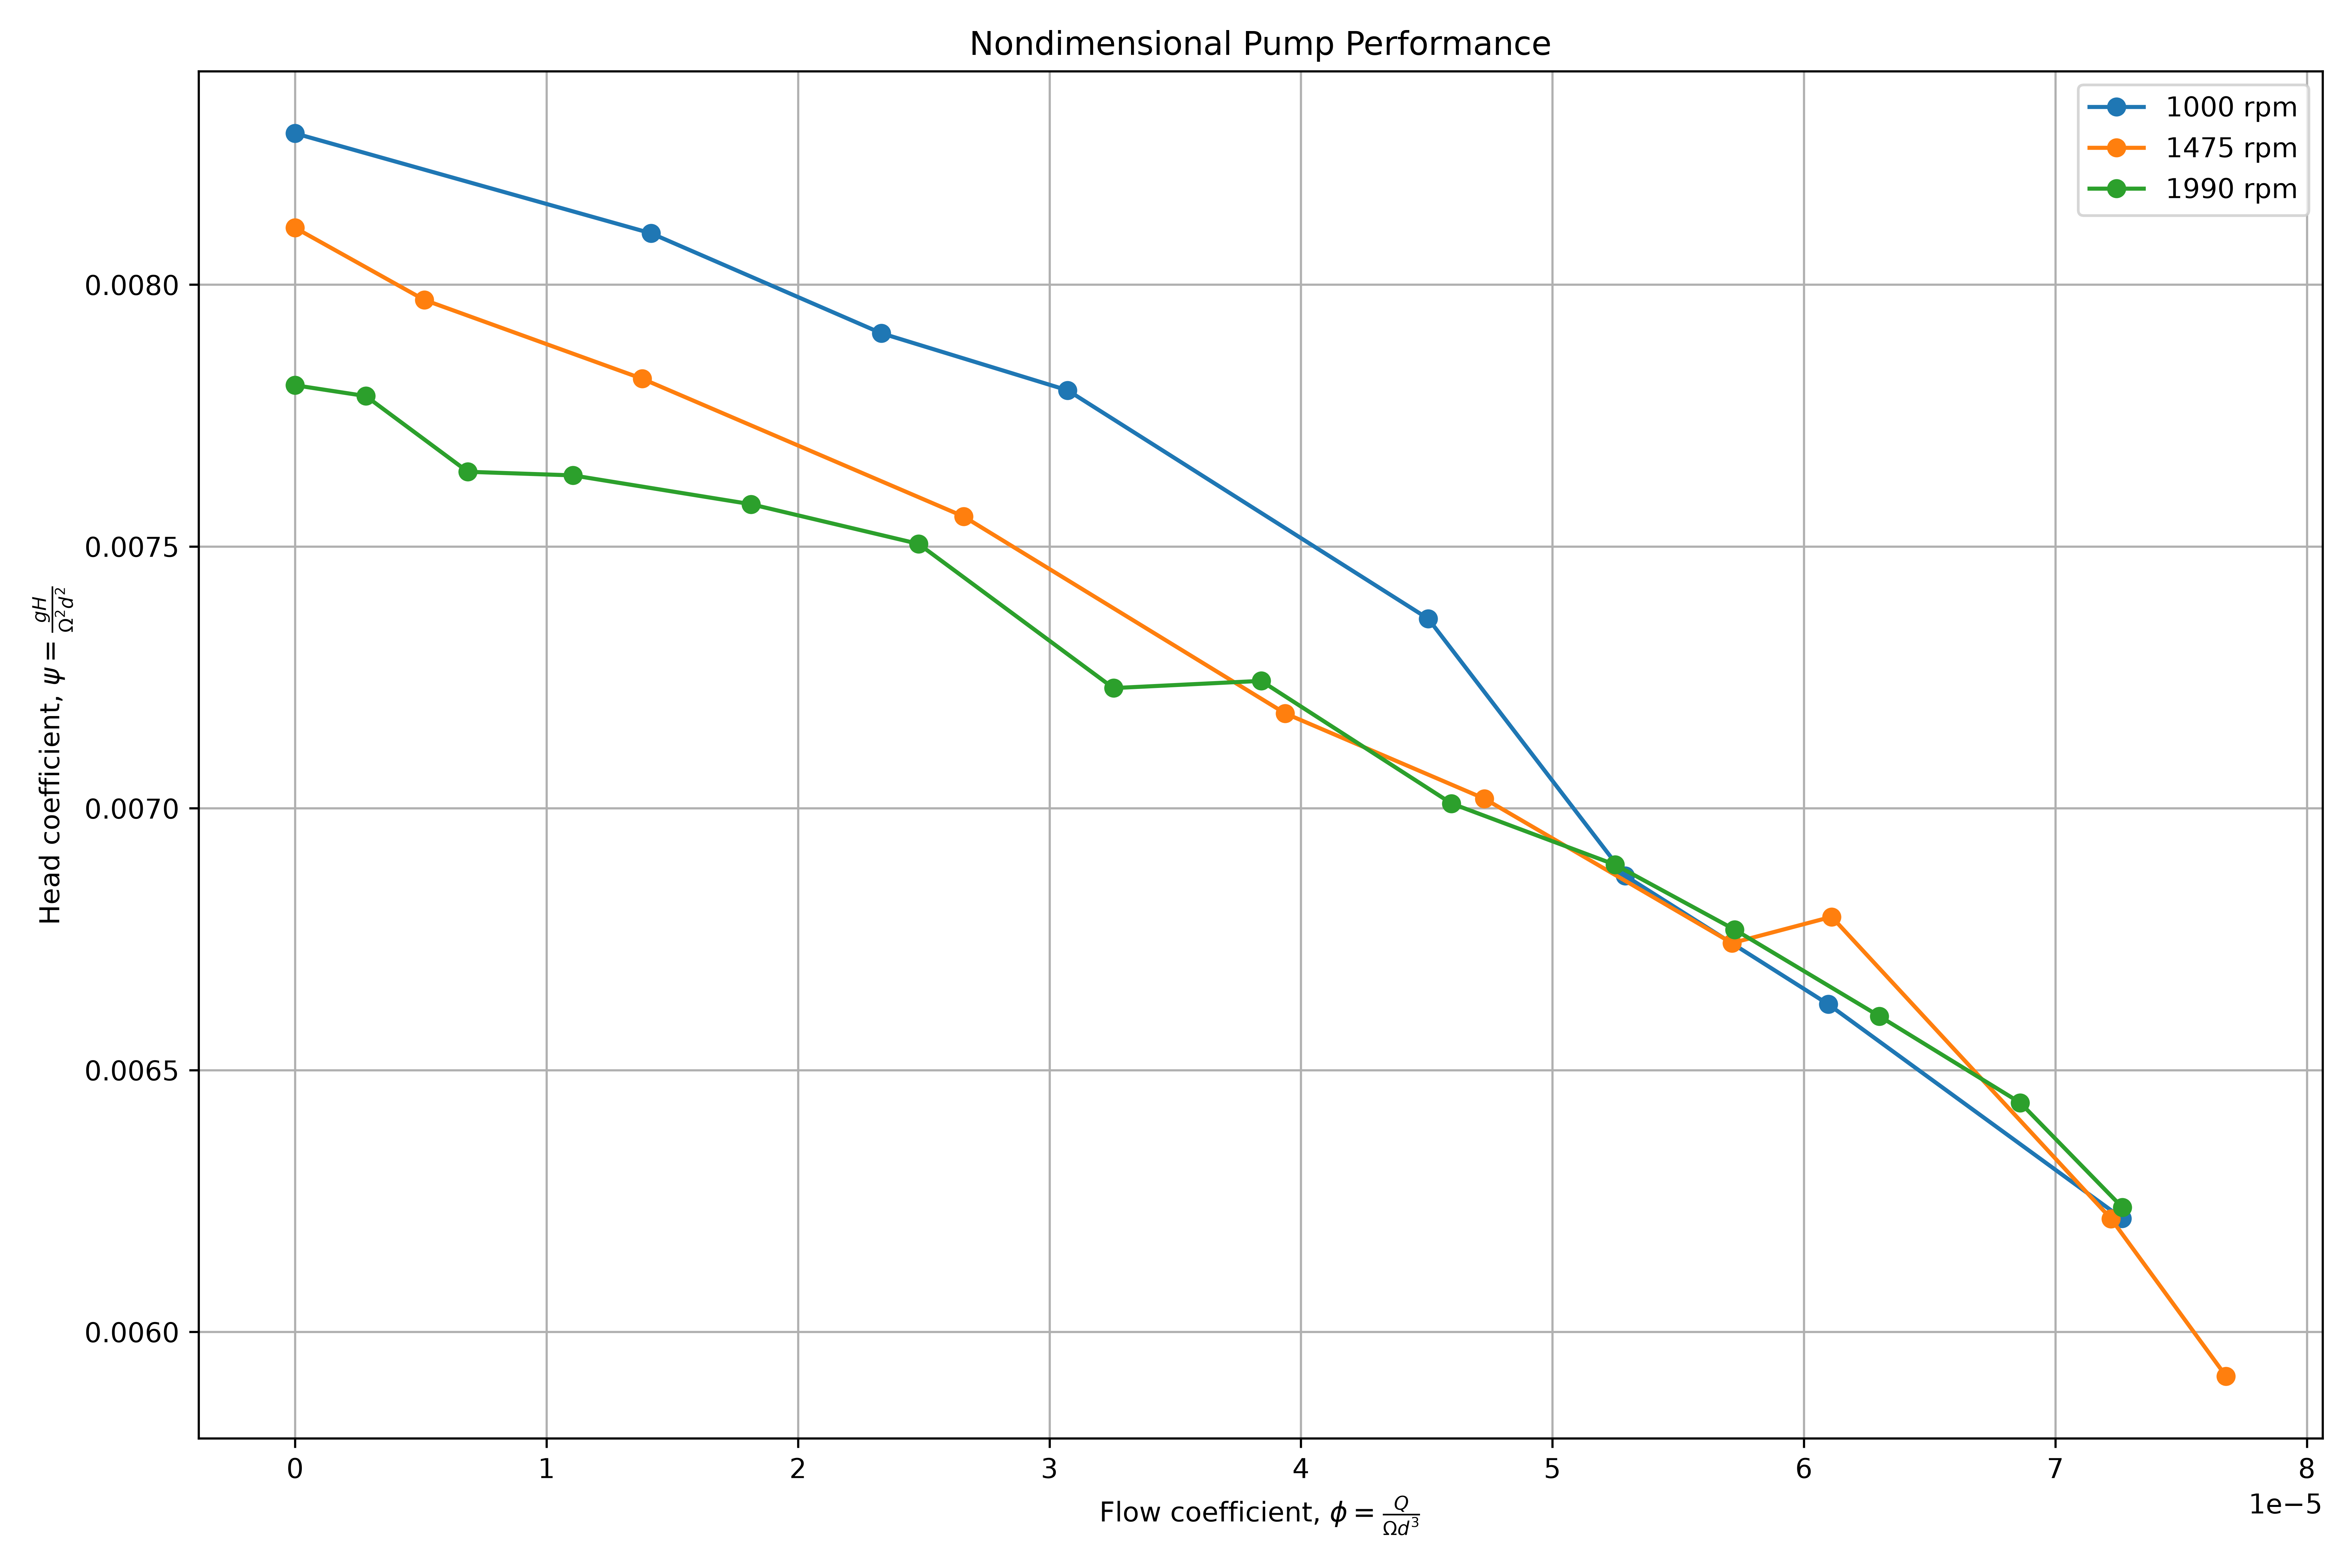
\includegraphics[width=0.75\textwidth]{../figures/pump_nondim.png}
    \caption{Nondimensional pump performance: head coefficient $\psi = gH/(\Omega^2 d^2)$ vs. flow coefficient $\phi = Q/(\Omega d^3)$ for three impeller speeds.}
    \label{fig:pump_nondim}
\end{figure}

\subsection*{Part (c)}
\textbf{Does your analysis appear to have identified the correct non-dimensional relationship? Why?}

Largely, yes. The three speed curves collapse quite closely onto a single curve $\psi = f(\phi)$ across most of the flow range, especially at moderate-to-high flow coefficients, which confirms that $\phi$ and $\psi$ are the dominant governing nondimensional groups for this pump. There is a small, systematic spread between the curves near shutoff (small $\phi$), where $\psi$ decreases slightly with increasing speed rather than collapsing exactly. This residual discrepancy is expected because part (a) explicitly neglected viscosity; in the real pump, viscous and internal leakage losses (captured by a Reynolds number $\text{Re} = \rho \Omega d^2/\mu$, which was assumed to be sufficiently large/negligible) are not perfectly self-similar across different speeds, since Reynolds number increases with $\Omega$. So the inviscid analysis captures the correct primary relationship, but the small imperfection in curve collapse reflects the secondary effect of viscosity that the analysis intentionally excluded.

\newpage

\section*{Problem 2}
\textbf{A gas of non-interacting particles of mass $m$ at temperature $T$ has density $\rho$, and internal energy per unit volume $\epsilon$.}

\subsection*{Part (a)}
\textbf{Using dimensional analysis, determine how $\epsilon$ must depend on $\rho, T,$ and $m$. In your formulation use $k_B =$ Boltzmann's constant, $h =$ Planck's constant, and $c =$ speed of light to include possible quantum and relativistic effects.}

First, we establish the fundamental dimensions for the variables:
\begin{itemize}[noitemsep]
    \item $[\epsilon] = M L^{-1} T^{-2}$
    \item $[m] = M$
    \item $[k_B] = M L^2 T^{-2} \Theta^{-1}$
    \item $[h] = M L^2 T^{-1}$
    \item $[c] = L T^{-1}$
    \item $[\rho] = M L^{-3}$
    \item $[T] = \Theta$
\end{itemize}

By choosing $m, k_B, h,$ and $c$ as repeating variables, we construct our three dimensionless groups ($\Pi_1, \Pi_2, \Pi_3$). 

For $\Pi_1$, containing $\epsilon$:
\begin{align*}
    \Pi_1 &= \epsilon m^a k_B^b h^c c^d \\
    M^0 L^0 T^0 \Theta^0 &= (M L^{-1} T^{-2})(M)^a (M L^2 T^{-2} \Theta^{-1})^b (M L^2 T^{-1})^c (L T^{-1})^d
\end{align*}
Solving the system of linear equations for the exponents yields $a = -4, b = 0, c = 3, d = -5$. Thus:
\begin{equation}
    \Pi_1 = \frac{\epsilon h^3}{m^4 c^5}
\end{equation}

For $\Pi_2$, containing $\rho$:
\begin{equation}
    \Pi_2 = \rho m^{-4} h^3 c^{-3} = \frac{\rho h^3}{m^4 c^3}
\end{equation}

For $\Pi_3$, containing $T$:
\begin{equation}
    \Pi_3 = T m^{-1} k_B^1 h^0 c^{-2} = \frac{k_B T}{m c^2}
\end{equation}

By the Buckingham Pi Theorem, $\Pi_1 = \mathcal{F}(\Pi_2, \Pi_3)$. Rearranging for $\epsilon$ gives:
\begin{equation}
    \epsilon = \frac{m^4 c^5}{h^3} \mathcal{F}\left(\frac{\rho h^3}{m^4 c^3}, \frac{k_B T}{m c^2}\right)
\end{equation}

\subsection*{Part (b)}
\textbf{Consider the limit of slow moving particles without quantum effects by requiring $c$ and $h$ to drop out of your dimensionless formulation. How does $\epsilon$ depend on $\rho$ and $T$? What type of gas follows this thermodynamic law?}

Assume a power-law form for the arbitrary function, $\mathcal{F}(\Pi_2, \Pi_3) = \gamma (\Pi_2)^\alpha (\Pi_3)^\beta$. Expanding this into the relation for $\epsilon$:
\begin{equation*}
    \epsilon = \gamma \rho^\alpha T^\beta k_B^\beta m^{(4 - 4\alpha - \beta)} h^{(3\alpha - 3)} c^{(5 - 3\alpha - 2\beta)}
\end{equation*}
To ensure $h$ and $c$ drop out, their exponents must equal zero:
\begin{align*}
    3\alpha - 3 &= 0 \implies \alpha = 1 \\
    5 - 3\alpha - 2\beta &= 0 \implies \beta = 1
\end{align*}
Substituting $\alpha = 1$ and $\beta = 1$ back into the expression yields:
\begin{equation}
    \epsilon = \gamma \frac{\rho k_B T}{m}
\end{equation}
The internal energy per unit volume depends linearly on density and temperature. This follows the thermodynamic law for a \textbf{classical ideal gas}.

\subsection*{Part (c)}
\textbf{Consider the limit of massless particles (i.e. photons) by requiring $m$ and $\rho$ to drop out of your dimensionless formulation of part a). How does $\epsilon$ depend on $T$ in this case? What is the name of this radiation law?}

Returning to the expanded power-law equation, we now require the exponents of $m$ and $\rho$ to be zero:
\begin{align*}
    \alpha &= 0 \\
    4 - 4\alpha - \beta &= 0 \implies \beta = 4
\end{align*}
Substituting $\alpha = 0$ and $\beta = 4$ back into the expression:
\begin{equation}
    \epsilon = \gamma \frac{k_B^4 T^4}{h^3 c^3}
\end{equation}
The internal energy per unit volume is proportional to $T^4$. This is known as the \textbf{Stefan-Boltzmann Law}.

\newpage

\section*{Problem 3}
\textbf{The vertical motion of a ship in water is governed by the $z$-component of the Navier-Stokes equation. The flow velocity far from the ship is given by $U$ and the length of the ship at the waterline is $l$.}

\subsection*{Part (a)}
\textbf{Non-dimensionalize the governing equation, the $z$-component of Navier-Stokes.}

We define characteristic scales to normalize the variables:
$z^* = \frac{z}{l}, \quad x^* = \frac{x}{l}, \quad y^* = \frac{y}{l}, \quad w^* = \frac{w}{U}, \quad u^* = \frac{u}{U}, \quad v^* = \frac{v}{U}, \quad t^* = \frac{tU}{l}, \quad p^* = \frac{p}{\rho U^2}$

Substituting these into the governing equation and dividing by the convective acceleration term ($\frac{U^2}{l}$) yields:
\begin{equation}
    \pd{w^*}{t^*} + u^*\pd{w^*}{x^*} + v^*\pd{w^*}{y^*} + w^*\pd{w^*}{z^*} = -\pd{p^*}{z^*} - \frac{g l}{U^2} + \frac{\mu}{\rho U l} \nabla^{*2} w^*
\end{equation}

\subsection*{Part (b)}
\textbf{What common non-dimensional parameters result?}

The resulting common non-dimensional parameters are:
\begin{itemize}
    \item Inverse Froude Number squared: $\frac{1}{Fr^2} = \frac{g l}{U^2}$
    \item Inverse Reynolds Number: $\frac{1}{Re} = \frac{\mu}{\rho U l}$
\end{itemize}

\subsection*{Part (c)}
\textbf{Assume you didn't have knowledge of the governing equation but knew that the $z$-velocity, $w$, was a function of $\rho, g, \mu, U,$ and $l$. Find the non-dimensional parameters using the Buckingham PI theorem.}

With 6 variables ($w, \rho, g, \mu, U, l$) and 3 fundamental dimensions ($M, L, T$), we choose $\rho, U, l$ as repeating variables to form $6 - 3 = 3$ dimensionless groups:
\begin{align*}
    \Pi_1 &= \frac{w}{U} \\
    \Pi_2 &= \frac{g l}{U^2} \quad \text{(Inverse Froude Number squared)} \\
    \Pi_3 &= \frac{\mu}{\rho U l} \quad \text{(Inverse Reynolds Number)}
\end{align*}
This matches the parameters found directly from the governing equation in part (b), as expected: pressure was not included among the given variables here, so no Euler-number-like group appears.

\subsection*{Part (d)}
\textbf{We wish to test a scaled model of a tanker ship at scale of 1/100 the actual size, is it practical to achieve dynamic similarity?}

It is \textbf{not practical}. Achieving dynamic similarity for surface vessels requires matching both the Froude number and the Reynolds number simultaneously. Matching the Froude number requires the model velocity to scale by $\sqrt{1/100} = 1/10$ of the actual velocity. However, matching the Reynolds number in the same fluid requires the model velocity to be $100$ times the actual velocity. These scaling requirements are contradictory.

\end{document}